\section{Source-level Debugging of Optimized Code}
A {\em source-level} (or {\em symbolic}) {\em debugger} is a program development tool that allows a programmer to monitor an executing program at the source-language level. Interactive mechanisms are typically provided to the user to halt/resume the execution at {\em breakpoints}, and to inspect the state of the program in terms of its source language. The importance of the design and use of these tools was already clear in the '60s~\cite{Evans66}.

\missing % DIRE DEI MOTIVI (vedi tesi Adl etc) - DEVO DIRE ANCHE LA COSA DI SINK E DCE?

As pointed out by Hennessy in his seminal paper from 1982~\cite{Hennessy82}, a classic conflict exists between the application of optimization techniques and the ability to debug a program symbolically. A debugger provides the user with the illusion that the source program is executing one statement at a time. On the other hand, optimizations preserve the semantic equivalence between optimized and unoptimized code, but normally alter the structure or intermediate results of a program.

Two problems surface when trying to symbolically debug optimized code~\cite{Adl-Tabatabai96,Jaramillo00}. First, the debugger must determine the position in the optimized code that corresponds to the breakpoint in the source code ({\em code location} problem). Second, the user expects to see the values of source variables at a breakpoint in a manner consistent with the source code, even though the optimizer might have 
deleted or reordered instructions, or values might have been overwritten as a consequence of the register allocator's choices ({\em data location} problem).

In general, there are two ways for a symbolic debugger to present meaningful information about the debugged optimized program~\cite{Wu99}. It provides {\em expected behavior} of the program if it hides the effect of the optimizations from the user and presents the program state consistent with what the user expects from the unoptimized code. It provides {\em truthful behavior} if it makes the user aware of the effects of optimizations and warns of possibly surprising outcomes.

Adl-Tabatabai observes in his PhD thesis that constraining optimizations or adding machinery during compilation to aid debugging do not solve the problem of debugging the optimized translation of a program, as the user debugs suboptimal code~\cite{Adl-Tabatabai96thesis}. Source-level debuggers thus need to implement techniques to recover expected behavior when possible, without relying on intrusive compiler extensions.

\subsection{Using \texorpdfstring{$\texttt{build\_comp}$}{build\_comp} for State Recovery}
%\subsection{Using  for State Recovery}
On-Stack Replacement has been pioneered in implementations of the SELF programming language to provide expected behavior with globally optimized code~\cite{Holzle92}. OSR shields the debugger from the effects of optimizations by dynamically deoptimizing code on demand. Debugging information is supplied by the compiler at discrete {\em interrupt points}, which act as a barrier for optimizations, letting the compiler run unhindered between them. Starting from the observation that our algorithms for generating OSR mappings (\mysection\ref{ss:osr-mapping}) do not place barriers for live-variable equivalent transformations, we investigated whether they could encode useful information for expected-behavior recovery in a source-level debugger.

As in most recent works on optimized code debugging, we focus on identifying and recovering scalar source variables in the presence of global optimizations. In LLVM, debugging information is inserted by the front-end as {\em metadata} attached to global variables, single instructions, functions or entire IR modules. Debugging metadata are transparent to optimization passes, do not prevent optimizations from happening, and are designed to be agnostic about the target debugging information representation (e.g., DWARF, stabs). Two intrinsics are used to associate IR virtual registers with source-level variables:
\begin{itemize}[itemsep=0pt,parsep=3pt]
 \item \mytt{llvm.dbg.declare} typically associates a source variable with an \alloca\footnote{\alloca\ is used to allocate space on the stack of the current function, to be automatically released when the function returns. Front-ends are not required to generate code in SSA form, but they can manipulate local variables created with \alloca\ using \load\ and \store\ instruction. Then the SSA form can be constructed using \memtoreg.} buffer;
 \item \mytt{llvm.dbg.value} informs that a source variable is being set to the value held by the virtual register.
\end{itemize}

\noindent We extended \tinyvm\ to reconstruct this mapping and also to indentify which program locations in the unoptimized IR version $f_{base}$ correspond to source-level locations for a function (as they would correspond to a possible user breakpoint location). An OSR mapping is then generated when OSR-aware transformation passes are applied to $f_{base}$ to generate the optimized version $f_{opt}$. For each location in $f_{opt}$ that might correspond to (i.e., have as OSR landing pad) a source-level location in $f_{base}$, we determine which variables live at destination are live also at source (and thus yield the same value), and which instead need to be reconstructed. We thus rely on the SSA form to identify which assignment(s) should be made in \reconstruct, as distinct assignments to source-level variables are represented by distinct IR objects. $\phi$-nodes at control-flow merge points of course can not be reconstructed, but our preliminary experimental investigation suggests that this might not be a huge issue in practice.

\missing % DIRE DI COME USARE QUESTE INFO (invisible breakpoints lo dico dopo?)

%As pointed out in~\cite{Adl-Tabatabai96}, compiler transformations cause {\em endangered} variables by either eliminating or moving assignments to source variables. 

\subsection{The \texorpdfstring{$\texttt{SPEC CPU2006}$}{SPEC CPU2006} Benchmarks}

\begin{table}[!t]
\begin{center}
\begin{small}
\begin{tabular}{ |c|r|r|r|r|r|r|r| }
\cline{3-8}
\multicolumn{2}{l|}{} & \multicolumn{6}{c|}{Functions} \\
\cline{3-8}
\multicolumn{2}{l|}{} & \multicolumn{1}{c|}{Total} & \multicolumn{2}{c|}{Optimized} & \multicolumn{3}{c|}{Endangered} \\
\hline
Benchmark & \multicolumn{1}{c|}{LOC} & \multicolumn{1}{c|}{$|F_{tot}|$} & \multicolumn{1}{c|}{$|F_{opt}|$}  & \multicolumn{1}{c|}{\tiny$\frac{|F_{opt}|}{|F_{tot}|}$} & \multicolumn{1}{c|}{$|F_{end}|$} & \multicolumn{1}{c|}{\tiny$\frac{|F_{end}|}{|F_{tot}|}$} & \multicolumn{1}{c|}{\tiny$\frac{|F_{end}|}{|F_{opt}|}$} \\ 
\hline
\hline
bzip2 & 8\,293 & 100 & 66 & 0.66 & 24 & 0.24 & 0.36 \\ 
\hline
gcc & 521\,078 & 5\,577 & 3\,884 & 0.70 & 1\,149 & 0.21 & 0.30 \\
\hline
gobmk & 197\,215 & 2\,523 & 1\,664 & 0.66 & 893 & 0.35 & 0.54 \\ 
\hline
h264ref & 51\,578 & 590 & 466 & 0.79 & 163 & 0.28 & 0.35 \\ 
\hline
hmmer & 35\,992 & 538 & 429 & 0.80 & 80 & 0.15 & 0.19 \\ 
\hline
lbm & 1\,155 & 19 & 17 & 0.89 & 2 & 0.11 & 0.12 \\ 
\hline
libquantum & 4\,358 & 115 & 85 & 0.74 & 9 & 0.08 & 0.11\\ 
\hline
mcf & 2\,658 & 24 & 21 & 0.88 & 11 & 0.46 & 0.52 \\ 
\hline
milc & 15\,042 & 235 & 157 & 0.67 & 34 & 0.14 & 0.22\\ 
\hline
perlbench & 155\,418 & 1\,870 & 1\,286 & 0.69 & 593 & 0.32 & 0.46 \\ 
\hline
sjeng & 13\,847 & 144 & 113 & 0.78 & 31 & 0.22 & 0.27 \\ 
\hline
sphinx3 & 25\,090 & 369 & 275 & 0.75 & 76 & 0.21 & 0.28 \\ 
\hline
\end{tabular} 
\end{small}
\end{center}
\caption{\label{tab:CS-debug-benchmarks} Characteristics of the C benchmarks from the \speccpu\ suite.} 
\end{table}

To capture a variety of programming patterns and styles from applications with different sizes, we have analyzed each method for each C benchmark in the \speccpu\ suite, applying the same sequence of OSR-aware optimization passes used in \mysection\ref{ss:bc-exp-setup} to the baseline IR version obtained with \clang\ \mytt{-O0} and then processed with \memtoreg. \mytable\ref{tab:CS-debug-benchmarks} reports for each benchmark the code size, the total number of functions in it, the number of functions amenable to optimization and, in turn, how many optimized functions report ``endangered'' user variables from a source-level debugger's perspective.

We observe that the fraction of functions that do not benefit from optimizations (i.e., $1-|F_{opt}|/F_{tot}|$) ranges from one tenth to one third of the total number of functions. For the optimized functions, the fraction of those that belong to $F_{end}$ - defined as the set of functions that require recovery of the expected behavior - ranges from $0.11$ (\mytt{libquantum}) to $0.54$ (\mytt{gobmk}).

\begin{table}[!ht]
\begin{center}
\begin{small}
\begin{tabular}{ |c|C{1.4cm}|C{1.4cm}|C{0.95cm}|C{0.95cm}|r| }
\cline{2-6}
\multicolumn{1}{l|}{} & \multicolumn{2}{c|}{Fraction of affected} & \multicolumn{3}{c|}{Endangered user vars} \\
\multicolumn{1}{l|}{} & \multicolumn{2}{c|}{program points} & \multicolumn{3}{c|}{per affected point} \\
\hline
Benchmark & $Avg_w$ & $Avg_u$ & $Avg$ & $\sigma$ & $Max$ \\ 
\hline
\hline
bzip2 & 0.17 & 0.12 & 1.22 & 0.55 & 5 \\
\hline
gcc & 0.25 & 0.22 & 1.13 & 0.31 & 14 \\
\hline
gobmk & 0.40 & 0.29 & 1.48 & 0.72 & 9 \\
\hline
h264ref & 0.45 & 0.55 & 1.69 & 1.23 & 14 \\
\hline
hmmer & 0.17 & 0.22 & 1.13 & 0.37 & 5 \\
\hline
lbm & 0.30 & 0.51 & 1.97 & 1.37 & 3 \\
\hline
libquantum & 0.13 & 0.10 & 1.06 & 0.17 & 2 \\
\hline
mcf & 0.35 & 0.32 & 1.00 & 0.00 & 1 \\
\hline
milc & 0.24 & 0.21 & 1.14 & 0.29 & 3 \\
\hline
perlbench & 0.37 & 0.35 & 1.16 & 0.36 & 8 \\
\hline
sjeng & 0.26 & 0.20 & 1.24 & 0.42 & 3 \\
\hline
sphinx3 & 0.29 & 0.31 & 1.19 & 0.44 & 6 \\
\hline
\hline
Mean & 0.28 & 0.28 & 1.28 & 0.52 & 6.08 \\
\hline
\end{tabular} 
\end{small}
\end{center}
\caption{\label{tab:CS-debug-affected-points} Fraction of program points with endangered user variables, and number of affected variables. The second and third column report weighted $Avg_g$ and unweighted $Avg_u$ average, respectively, of the fraction of such points for functions in $F_{end}$. We use the number of IR instructions in the unoptimized code as weight for computing $Avg_w$, and consider only IR program points corresponding to source-level locations. We then show mean, std deviation, and peak number of endangered variables at such points.} 
\end{table}

\mytable\ref{tab:CS-debug-affected-points} reports figures that we have collected for functions in $F_{end}$. We observe that on average, more than one in every four program points there is at least a user variable whose source-level value might not be reported correctly by a debugger. For most functions in the benchmarks, the average number of affected user variables at such points ranges between $1$ and $2$, although for some benchmarks we observe high peak values at specific points (e.g., $9$ for \mytt{gobmk} and $14$ for \mytt{gcc} and \mytt{h264ref}).

To investigate possible correlations between the size of a function and the number of user variables affected by source-level debugging issues, we analyzed the corpus of functions for the three largest benchmarks in our suite, namely \mytt{gcc}, \mytt{gobmk}, and \mytt{perlbench}. \myfigure\ref{fig:CS-debug-ratio} shows scatter plots in which each point represents a function: the horiziontal position is given by the number of IR instructions in the unoptimized code, while the vertical position by the sum of the number of endangered user variables across program points corresponding to source-level locations.

\begin{figure}[!t]
\begin{center}
\centerline{
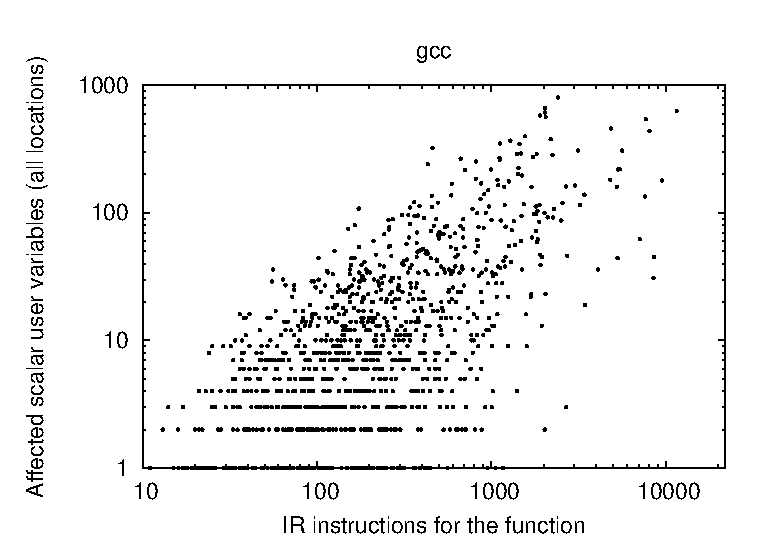
\includegraphics[width=0.45\textwidth]{figures/CS-debug-tot-dead/tot-dead-gcc-logscale.eps}
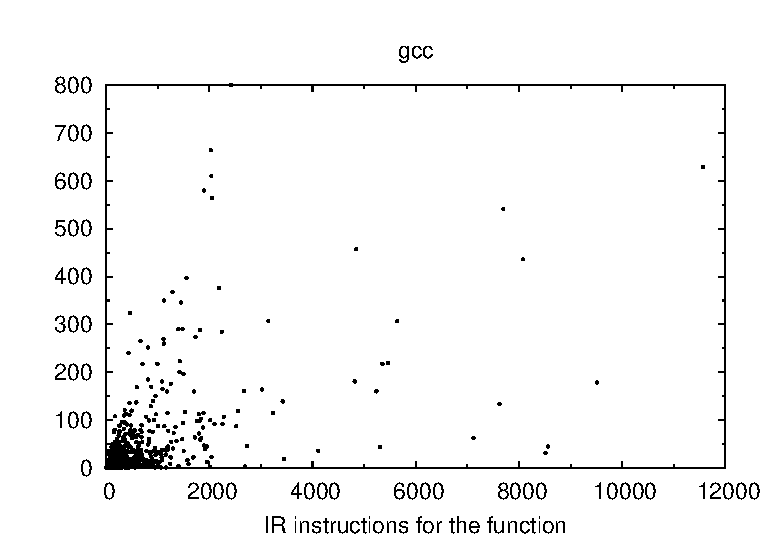
\includegraphics[width=0.45\textwidth]{figures/CS-debug-tot-dead/tot-dead-gcc-linear.eps}
}
\vspace{2mm}
\centerline{
\includegraphics[width=0.45\textwidth]{figures/CS-debug-tot-dead/tot-dead-gobmk-logscale.eps}
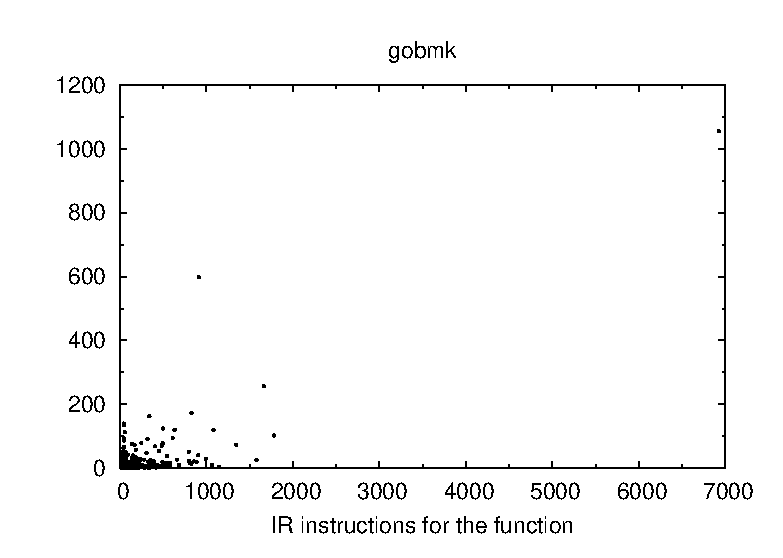
\includegraphics[width=0.45\textwidth]{figures/CS-debug-tot-dead/tot-dead-gobmk-linear.eps}
}
\vspace{2mm}
\centerline{
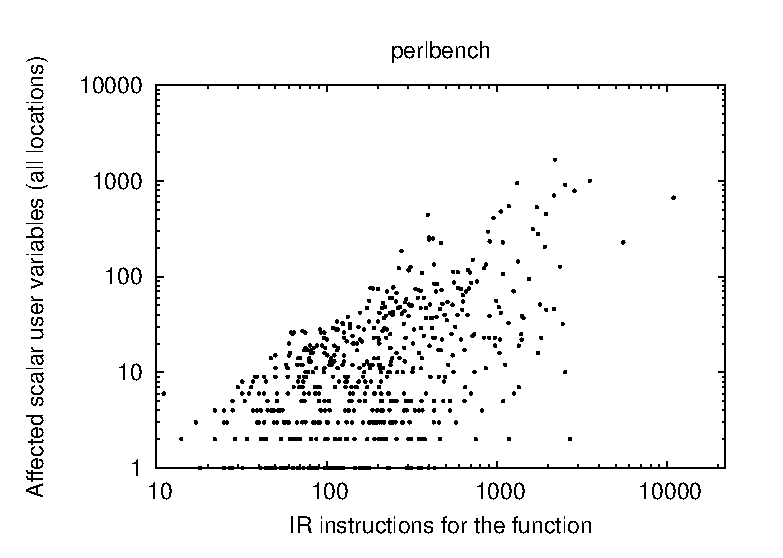
\includegraphics[width=0.45\textwidth]{figures/CS-debug-tot-dead/tot-dead-perlbench-logscale.eps}
\includegraphics[width=0.45\textwidth]{figures/CS-debug-tot-dead/tot-dead-perlbench-linear.eps}
}
\caption{\protect\label{fig:CS-debug-tot-dead} Scatter plot of the total number of scalar user variables that are endangered by optimizations across program points. The position on the horizontal axis is determined by the number of instructions in each function's unoptimized version. For each selected benchmark we report both a log-log (left) and a linear (right) plot.}
\end{center}
\end{figure}

The log-log plots for \mytt{gcc} may suggest a trendline such that larger functions would typically have a large number of affected variables. However, this trend is less pronounced in \mytt{perlbench}, and nearly absent from \mytt{gobmk}. Linear plots should provide a better visualization of what happens for larger functions and for functions with a higher total number of affected variables. We can safely conclude that, although larger functions might be more prone to source-level debugging issues, these issues frequently arise for smaller functions as well.

\subsection{Experimental Results}
We have evaluated the ability of \buildcomp\ to correctly reconstruct the source-level expected value for all the endangered user variables in the \speccpu\ experiments. For each function, we measured the {\em average recoverability ratio}, defined as the average across all program points corresponding to source-level locations of the ratio between recoverable and endangered user variables for a specific point. Two versions of \reconstruct\ can be useful in this setting: $live_{(e)}$ and $avail$ (\mysection\ref{ss:BC-implementation}).

$live_{(e)}$ can be used in a debugger that can evaluate expressions over the current program state, such as \gdb\ or LLDB\footnote{As LLDB is tightly coupled with the rest of the LLVM infrastructure, it can also utilize its JIT to run and evaluate arbitrary code. \gdb\ can typically evaluate complex expressions as well.}. In fact, this version of \reconstruct\ needs only to access the live state of the optimized program at the breakpoint.

$avail$ can be integrated in a debugger using {\em invisible} breakpoints to spill a number of non-live available values before they are overwritten. Invisible breakpoints are indeed largely employed in source-level debuggers (e.g., ~\cite{Zellweger83,Wu99,Jaramillo00}). Using spilled values and the current live state, expected values for endangered user variables can be reconstructed as for $live_{(e)}$. Alternatively, in a virtual machine with a JIT compiler and an integrated debugger, the runtime might decide to recompile a function when the user inserts a breakpoint in it, artificially extending the liveness range for the values that will be needed by \buildcomp.

\begin{figure}[!ht]
\begin{center}
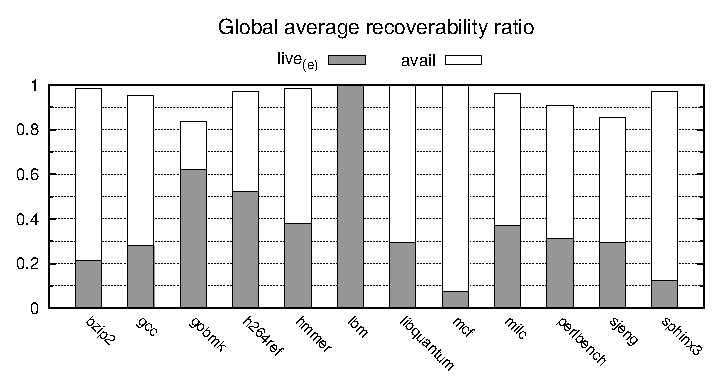
\includegraphics[width=0.8\textwidth]{figures/CS-debug-ratio/CS-debug-ratio.eps}
\caption{\protect\label{fig:CS-debug-ratio} Global average recoverability ratio, defined as weighted average of each function's average recoverability ratio. We used the number of unoptimized LLVM IR instructions as weight.}
\end{center}
\end{figure}

\myfigure\ref{fig:CS-debug-ratio} shows for each benchmark the global average recoverability ratio achieved by $live_{(e)}$ and $avail$ on the set of affected functions $F_{end}$. To compute the global average, the average recoverability ratio for each function has been weighted using the size of the unoptimized function as weight. We observe that $avail$ performs particularly well on all benchmarks, with a global ratio higher than $0.95$ for half of the benchmarks, and higher than $0.9$ for $10$ out of $12$ benchmarks. In the worst case (\mytt{gobmk}), we observe a global ratio slightly higher than $0.83$. Results thus suggest that \buildcomp\ can be effective in recovering a vast majority of expected values for endangered source-level variables.

\begin{table}[!ht]
\begin{center}
\begin{small}
\begin{adjustbox}{width=0.925\textwidth}
\begin{tabular}{ |c|c|c|c|c|c|>{\centering}p{0.58cm}|c|c|c|c|c|c||c| }
\cline{2-14}
\multicolumn{1}{c|}{} & \rot{bzip2} & \rot{gcc} & \rot{gobmk} & \rot{h264ref} & \rot{hmmer} & \rot{lbm} & \rot{libquantum\hspace{0.5em}} & \rot{mcf} & \rot{milc} & \rot{perlbench} & \rot{sjeng} & \rot{sphinx3} & \rot{Mean} \\
\hline
%$avg$ & 2.29 & 1.99 & 0.38 & 3.48 & 1.95 & 0 & 2.00 & 1.82 & 1.68 & 3.14 & 1.45 & 1.67 & 1.82 \\
%$\sigma$ & 3.20 & 4.51 & 1.23 & 8.09 & 2.33 & 0 & 3.12 & 0.87 & 1.93 & 4.60 & 1.26 & 2.05 & 2.77 \\
%\hline
%C & 12.00 & 77.00 & 12.00 & 88.00 & 9.00 & 0.00 & 10.00 & 3.00 & 8.00 & 32.00 & 5.00 & 11.00 & 22.25 \\
$frac$ & 0.71 & 0.72 & 0.16 & 0.71 & 0.70 & - & 0.67 & 1.00 & 0.76 & 0.66 & 0.77 & 0.72 & 0.69 \\
\hline
$avg$ & 3.24 & 2.77 & 2.31 & 4.90 & 2.79 & - & 3.00 & 1.82 & 2.19 & 4.76 & 1.88 & 2.31 & 2.91 \\ 
\hline
\hline
$\sigma$ & 3.38 & 5.12 & 2.22 & 9.23 & 2.33 & - & 3.46 & 0.87 & 1.94 & 4.94 & 1.12 & 2.08 & 3.34 \\
\hline
\end{tabular} 
\end{adjustbox}
\end{small}
\end{center}
\caption{\label{tab:CS-debug-dead-avail} Available values to preserve when using $avail$. For functions that require to preserve at least one value, we report the fraction $frac$ of $|F_{end}|$ they cumulatively account for, the average number $avg$ of values to preserve across such functions, and the associated standard deviation $\sigma$.
} 
\end{table}

To estimate how many values should be preserved - through either invisible breakpoints or recompilation - to use $avail$ in a debugger, we collected for each function the ``keep'' set of non-live available values to save to support deoptimization across all program points corresponding to source-level locations. We then computed the mean and the standard deviation for the size of this set on all functions in $F_{end}$. Figures reported in \mytable\ref{tab:CS-debug-dead-avail} show that typically a third of the functions in $F_{end}$ do not require any values to be preserved. For the remaining functions, on average $2.91$ values need to be preserved, with a peak of $4.90$ observed for \mytt{h264ref}.

Observe that values in the keep set do not necessarily neeed to be preserved simultaneously at all program points same points: indeed, some of them might be required only in certain regions of a function. In the debugging practice, what typically happens is that values are saved using an invisible breakpoint before they are overwritten, and deleted as soon as they are no longer needed~\cite{Jaramillo00}. For the recompilation-based approach, on the other hand, numbers reported in \mytable\ref{tab:CS-debug-dead-avail} should be interpreted as a pessimistic upper-bound for register pressure increase.

\subsection{Discussion}


%However, when attempting to debug optimized programs, most debuggers may give misleading information about the value of variables at breakpoints.
%Hence, the programmer has the difficult task of attempting to unravel the optimized code 